% On TexStudio
% PdfLatex
% Biber
%
\RequirePackage{luatex85}% TeXLive 2017 fix for \geometry

\documentclass[letterpaper]{kdp}


\usepackage{graphicx} 
\usepackage{amsmath,amssymb,amsfonts,xcolor,amsthm}
\usepackage{soulutf8}

\usepackage{algorithm,algorithmic}
\usepackage{stfloats}
\usepackage{cite}
\usepackage{float}
\usepackage{graphicx}         
\usepackage{textcomp}
\usepackage[export]{adjustbox}
\usepackage{longtable}
\usepackage{balance}
\usepackage[numbers]{natbib}
\usepackage{listings}
\usepackage{matlab-prettifier}


\usepackage{tikz}
\usetikzlibrary{mindmap,trees}
\newcommand{\mypaper}{article}
\allowdisplaybreaks
\newtheorem{lemma}{{\bf Lemma}}
\usepackage{tabularx}
\usepackage{boldline}
\usepackage[normalem]{ulem}

\usepackage{titlepic}
\usepackage{background}



\newcommand{\pycode}[1]{\lstinline[language=Python, style=Matlab-editor]|#1|}
\newcommand{\code}[1]{\lstinline[basicstyle=\ttfamily\bfseries\color{brown}]|#1|}
\newcommand{\matlabcode}[1]{\lstinline[language=Matlab,style=Matlab-editor]|#1|}


% Set up the background image
\backgroundsetup{
  scale=1,
  color=black,
  opacity=0.8, % Change opacity as needed
  angle=0,
  vshift=0cm,
  hshift=0cm,
  contents={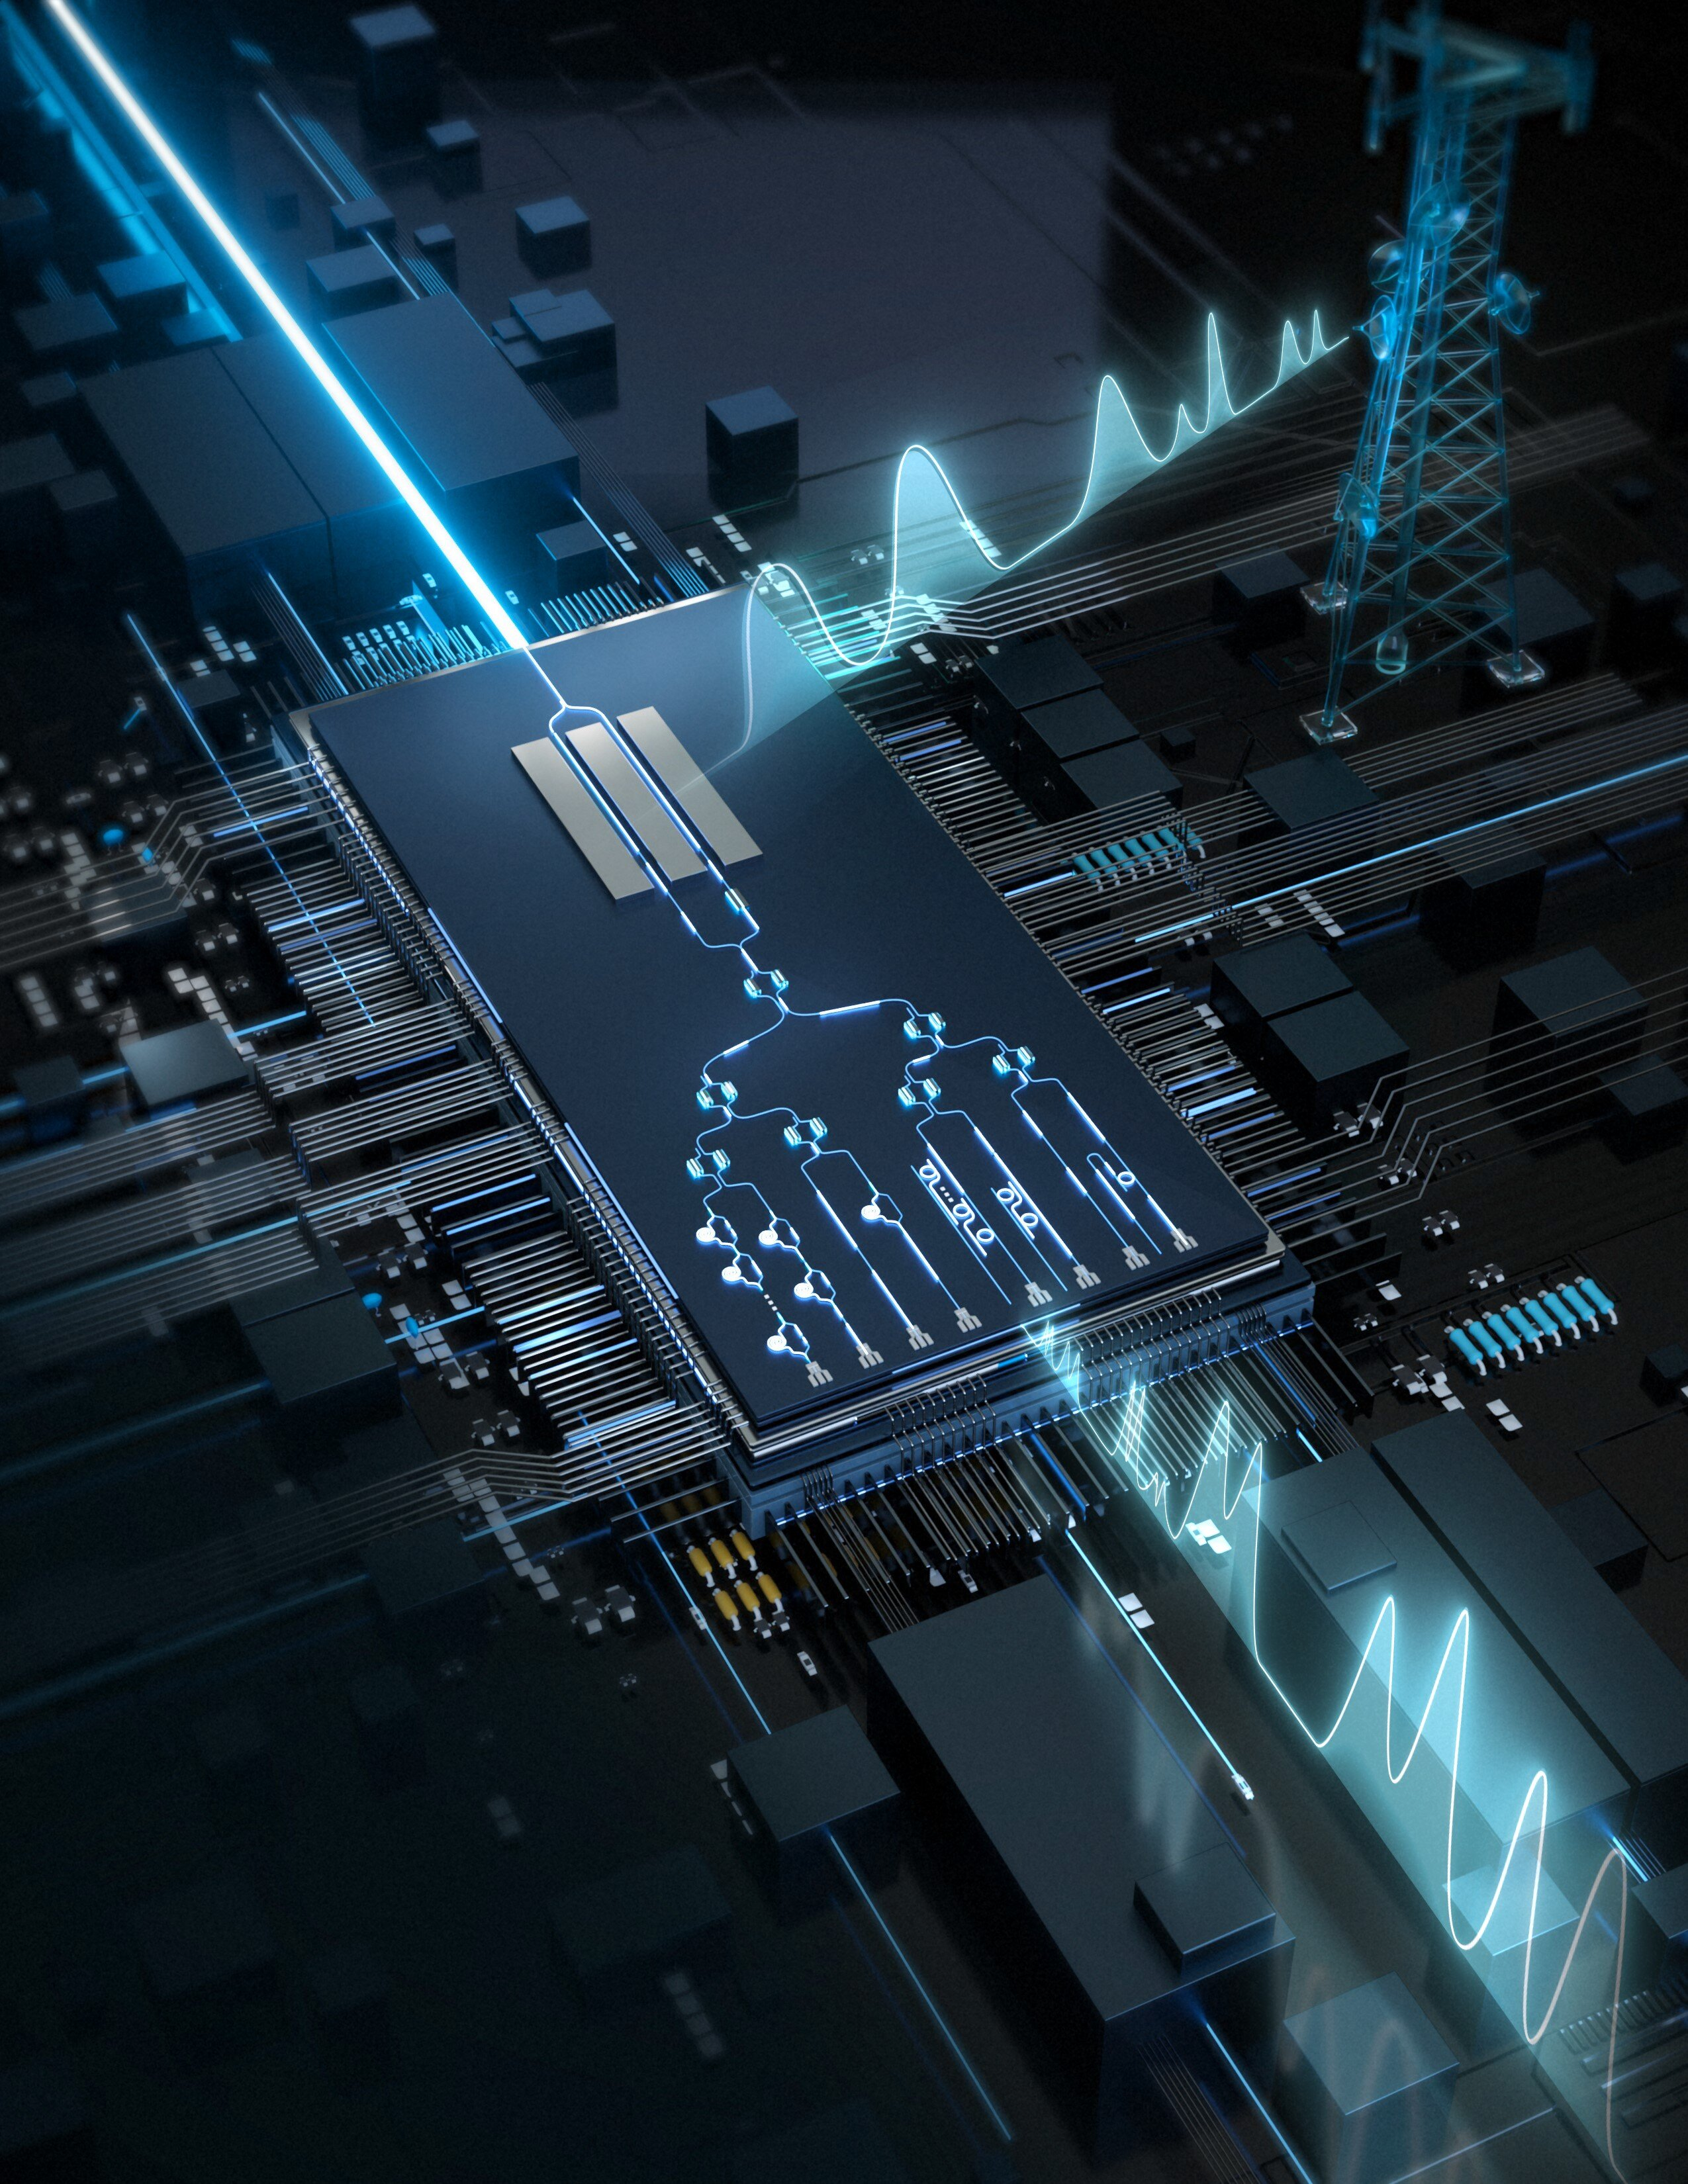
\includegraphics[width=\paperwidth,height=\paperheight]{title-page.jpg}} % Change to your image file
}

\usepackage{geometry}



\begin{document}
\pagenumbering{gobble}

\begin{titlepage}
    \color{yellow}
    \centering
    \vspace*{1cm}
    
    \vspace{1cm}
        
    {\fontsize{29pt}{29pt}\selectfont \bfseries KDP Book Title\\\vspace*{0.25cm}Some Subtitle}\\[0.4cm]
    
    \color{white}
    \vspace*{1.5cm}
    \textit{\fontsize{15pt}{15pt}\selectfont \bfseries author name \& another author name}\\
    \vspace*{0.5cm}
    \textit{\fontsize{14pt}{14pt}\selectfont affiliation}
    

    
\end{titlepage}
\backgroundsetup{contents={}}

\clearpage
\tableofcontents
\newpage

\pagenumbering{arabic}

\chapter{First Chapter}

\section{First Section}


\section{Other Section}

The content of this section ....



\bibliographystyle{IEEEtranN}
\bibliography{IEEEabrv, refs}
\end{document}
